In an attempt to create a model based controller that can be applied to the soft robotic actuator, the developed non-linear model should first be validated. This is done by using a planar 2 degree-of-freedom soft robot. This robot has a translational and rotational degree of freedom.  Rotation is only dependent on the difference in bellow length, not absolute bellow length. To measure rotation, an Inertial Measurement Unit (IMU) is connected at the tip of the robot. The position of the bellows can be tracked with a camera set-up. From this data, elongation and curvature of each individual bellow can extracted. Being able to measure/determine both degrees-of-freedom allows us to validate the dynamic model. The best way of validating the model is using a 


\section{Model validation for the planar soft actuator}


\subsection{Measuring Devices}


\subsubsection{Inertial Measurement Device (IMU)}


Discuss what the IMU does, how it works, where and why it is connected at the top, complementary filter



\subsubsection{Vision system}

Discuss the vision system, 2D motion tracking.



\subsection{Model validation approach}

The model will be validated using a free swing type





\subsection{Pressure control}

In order to carry out a validation a pressure control strategy needs to be established.  


\begin{figure}[H]
    \centering
    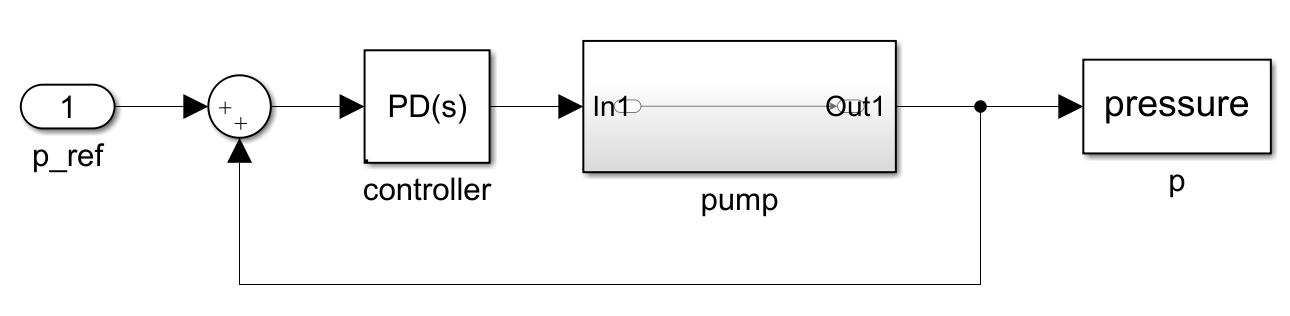
\includegraphics[width = \linewidth]{Figures/Chapter2/pressurecontrol.png}
    \caption{Control lay-out for pressure control}
    \label{fig2:pcontrol}
\end{figure}







\subsection{Kinematic description of the planar robot}

Define vector $\textit{\textbf{q}}$ which captures the length of each bellow as:

\begin{equation}
    \textit{\textbf{q}} = \begin{bmatrix} q_1 , q_2 \end{bmatrix} ^\top
\end{equation}

With the constant curvature approach, the center length of the planar robot can be determined as:


\begin{equation}
    \textit{\textbf{k}}(\textit{\textbf{q}}) = \begin{bmatrix}  \kappa(\textit{\textbf{q}}) \\ l(\textit{\textbf{q}}) \end{bmatrix} = \begin{bmatrix} \frac{q_1-q_2}{(q_1+q_2)r_b} \\ \frac{q_1+q_2}{2} \end{bmatrix}
    \label{eq2:ccmapping}
\end{equation}

The IMU is able to measure the rotation of the tip of the actuator, while with the vision system the coordinates of the center of the actuator can be tracked in Cartesian 2D space. With the circle segment theory the measured $x$ and $y$ coordinates can be transformed to the curvature and length of the actuator tip with the following mapping:

\begin{equation}
    \textit{\textbf{k}}(\textit{\textbf{x}}) = \begin{bmatrix} \kappa(\textit{\textbf{x}}) \\ l(\textit{\textbf{x}}) \end{bmatrix} = \begin{bmatrix} \frac{2 \sin (\frac{1}{2}\varphi)}{\sqrt{x^2+y^2}} \\
    \frac{\varphi \sqrt{x^2+y^2}}{2 \sin(\frac{1}{2}\varphi)} \end{bmatrix}
\end{equation}

Now $\varphi$ is and $l$ are determined with the IMU and vision system, respectively. The bellow lengths $q_1$ and $q_2$ can be calculated using relation \ref{eq2:ccmapping} as:

\begin{equation}
    q_1 = r_B \varphi + \frac{\varphi \sqrt{x^2+y^2}}{2 \sin(\frac{1}{2}\varphi)}
\end{equation}

\begin{equation}
    q_2 = -r_B \varphi + \frac{\varphi \sqrt{x^2+y^2}}{2 \sin(\frac{1}{2}\varphi)}
\end{equation}

Where $r_B$ is the distance from the center of the bellow to the center of the actuator.


\subsection{Pump pressure relation}





\subsection{Experimental set up}


The set-up as is present in the lab can be used. How









\subsection{Results}

In this section a comparison between the dynamic model and experiment should be made. That means the a comparison between the model's rotation and elongation for a given pressure/force.  


\subsection{Model adaptations}


%\begin{equation}
%    \textit{\textbf{q}} = \begin{bmatrix}
%    q_1 & q_2 
%\end{bmatrix} ^\top
%\end{equation}


